\section{Task Analysis}

We investigated into the design needs for collaborative information analysis in four ways. First, we examined existing works that already conducted empirical user studies of information analysts, including \cite{Chin2009,Borge2012,Borge2014,Carroll2013,Pirolli2005} conducted a paper prototype study [1], [2], in which we observed 22 teams investigating a crime scenario. In the task, teams of participants spent about four hours in which they identify, analyze and evaluate conclusions from 222 propositions embedded in a set of problem documents. This study sheds light on team process patterns, collaboration breakdowns, and possible technical support teams need. The second study observed student training in an intelligence analysis course in a U.S. university. The course was designed to train students to become professional intelligence analysts. In the course, students learned theories of analysis (e.g. bottom-up analysis vs. top-down analysis, and concepts of hypothesis, assumption, and evidence), analytic techniques (e.g. Analysis of Competing Hypotheses (ACH) and Link Analysis), as well as the state-of-the-art tools to support the implementation of those techniques (e.g. PARC ACH [3] and Analyst’s Notebook [4]). We observed how they applied these techniques to solving an intelligence project. This study suggests current practices in intelligence analysis, challenges in current practices, and potential technical support needed.  Below we summarized our findings.

\subsection{Major activities: data modeling, data analysis, and hypothesis development}

Participants performed three major activities: data modeling, data analysis, and hypothesis generation. A typical workflow is shown in Figure~\ref{fig:workflow}. Analysis started from a collection of documents, including intelligence reports, witness reports, media news, etc. As they read through the documents, they highlighted important evidence, made annotations, and extracted them in a separate file for evidence record. We call this process “data modeling”, as analysts modeled textual documents into structured evidence entities, including suspects, events, locations, resources (e.g. money, weapon, vehicle), and relationships (e.g. social relationships, financial transactions). Entities are held in an Information Extraction and Weighting (IEW) Table, in which they listed evidence and weighed its face value and alternative value against analytic problems.
To examine patterns between evidence, analysts utilized various tools to visualize and synthesize evidence. Such data analysis was fed into hypothesis development, and fit into a best hypothesis. We will discuss data analysis and hypothesis development in the following separate sections. Note that we describe the three activities in a linear fashion for the sake of writing, but analysis could be performed in any order, and most commonly, in an iterative approach.
One problem in the workflow is a breakdown between activities. Systems that support intelligence analysis are aimed at a single activity and therefore only support part of the overall analysis workflow. This imposes a clear boundary between each of these activities on the analysts. For example, IEW helps structure evidence modeling, but does not extend utilization of evidence to hypothesis generation; ACH assumes that data has been modeled, and that relevant evidence can be adduced appropriately to various hypotheses, but provides no structured support for either. The unintended boundary between phases has the consequence that data modeled in one software cannot be effectively utilized in hypothesis development in another system. And analysts have to handoff, often via replicating the data in the new system, information between software systems, making it difficult to revisit and revise the data model.

\begin{figure}
\centering
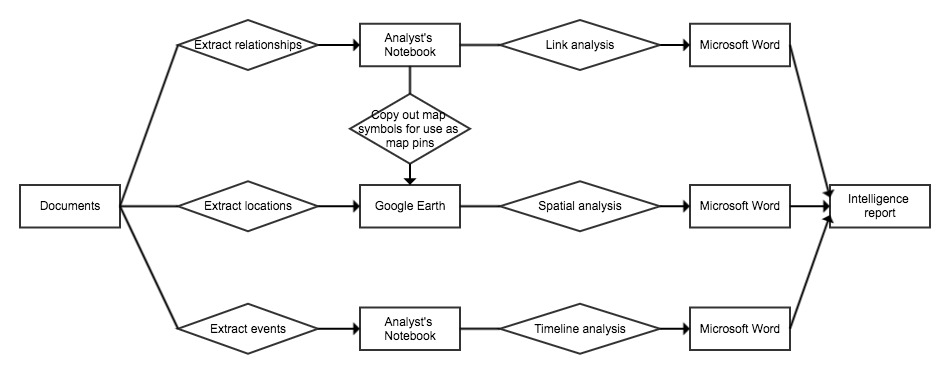
\includegraphics[width=3.00000in]{./workflow.jpg}
\caption{Participant reported intelligence analysis workflow)\label{fig:workflow}}
\end{figure}

\subsection{Multi-dimensional evidence marshaling}

In data analysis, analysts explored multiple dimensions of data. Participants explored these data in different visualization tools. For example, they modeled events in Analyst’s Notebook’s timeline tool to identify sequential patterns. Social relationships were represented in the network tool in Analyst’s Notebook for link analysis. To do spatial analysis, they extracted locations and created pins on Google Earth. The need for multiple analytic views is also observed in the paper prototype study, where participants spontaneously created artifacts such as table, maps, network, and calendar.
Evidence marshaling is a common technique to assemble pieces of evidence and tie them to hypotheses and assertions. The technique connects bits of information together and provides a complete picture of the story. Without tool support, analysts often do a simple, informal marshaling in their mind. With an elaborate computer-based method, analysts can, for example, coordinate events along a timeline, and organize evidence into stories about typical topics (e.g. what, when, where, who, and how).
One problem participants encountered was the inconsistency between representations of different tools. For example, the symbols representing locations in Analyst’s Notebook were different from those used in Google Earth. The inconsistency added difficulty to view interpretation. Our participants were aware of the problem and a routine practice in their workflow (as shown in Figure~\ref{fig:workflow}) was to manually copy out symbols in Analyst’s Notebook and import them into Google Earth, which is apparently a disjointed user experience. Another problem was the lack of support in coordinated view exploration. While examining individual views are is of value, patterns are more likely to be revealed by marshaling views together. For example, analysts would create a spatial filter on the map and investigate events that happened within a specific geographic area. However, in the current workflow, views are separate and self closed in their own tools.

\subsection{Hypothesis development}

Analysts generate multiple hypotheses and find evidence to confirm or disconfirm them. A common technique to evaluate hypotheses is Analysis of competing hypotheses (ACH) [5]. ACH emphasizes a rational, transparent process of hypothesis analysis. The steps include identifying a complete set of hypotheses, identifying all pieces of evidence, assessing the diagnostic value of each evidence against each hypothesis, and drawing conclusions of the likelihood of hypotheses. ACH guarantees an appropriate analytic process and increases the chance to avoid common analytical pitfalls such as confirmation bias.
In practice, however, we found students rarely came up with a complete set of hypotheses in the very beginning. Instead, they began with reading documents and got familiar with the suspects. They would propose a hypothesis in the process of extracting and marshaling evidence. They would share their hypothesis with teammates or document it in a note. With evidence accumulating, the team collaboratively refine the existing hypotheses, and propose alternative hypotheses. The process was iterative, with hypotheses constantly being refined and evolved.
ACH demands a high expertise bar for analysts. Users are required to identify a complete set of mutually exclusive hypotheses at the very beginning, which is difficult for people with little expertise and experience in the domain. Further, hypotheses tend to evolve as analysis proceeds. A hypothesis valid in the beginning may no longer be of value later, or two seemingly separate hypotheses in an early stage of analysis could be combined in a way to better explain the situation later on. The assumption ACH makes that all hypotheses and evidence are identified and set in the very beginning limits the dynamic evolvement and development of analysis.

\subsection{Collaboration}

While collaboration is critical in intelligence analysis, most supporting tools (e.g. PARC ACH and Analyst’s Notebook) are not designed for collaborative use. We observed several pain points in participants’ collaboration. For example, participants were unable to contribute simultaneously. Working on the same file would cause conflict. Collaborators had to wait when one teammate was working on the tool. This was known as production blocking [@Diehl1987a], in which individual performing a task became a bottleneck of team process. To work around the issue, participants often divided their work by tools: each person picked a tool and then created and analyzed an artifact with the tool on their own. This had the consequence that findings and hypotheses be made without integrating collective efforts and diverse knowledge. Participants shared their findings only after they already had a conclusion, which was obviously opposed to collaboration.
Analysts coordinated work outside the tool, by manually sharing documents or graphs through email or cloud storage service (e.g.~Dropbox). As shown in Figure~\ref{fig:workflow}, analysts manually took screenshots of views and copied them into Microsoft Word. This has the consequence multiple views exist in distrubited locations, adding burden to analyst’s limited cognition. Analysts could easily overlook certain aspect when they were evaluating hypotheses. The interactive views become static images, making it impossible for collaborators to further explore. Worse, if data model changes, analysts must manually update the views, resulting multiple versions of views.
